\documentclass[10pt]{beamer}
\usepackage{xeCJK}
\usepackage{graphicx}
\usepackage{booktabs}
\usepackage{listings}
\usepackage{multirow}
\usepackage{mathtools}
\usepackage{ulem}
\usefonttheme[onlymath]{serif}
\usetheme{metropolis}
\setbeamercolor{footnote mark}{fg=blue}% set footnote color in beamer
\setbeamerfont{footnote}{size=\tiny}
\begin{document}
	\title{杂谈}
	\date{\today}
	\author{huhao}
	\maketitle
	\clearpage
	\begin{frame}
	
		隔离期间,讲点简单的让大家放松一下。\sout{(下图当事人已打码)}
		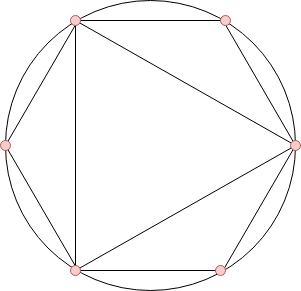
\includegraphics[width=0.7\textwidth]{1.JPG}

	\end{frame}
	\begin{frame}
		\frametitle{行列式相关I}

		行列式定义:

		$$
		\sum_i \mathrm{sgn}(i)\prod_j a_{j,i_j}
		$$

		其中$\mathrm{sgn}$为逆序对数。

	\end{frame}
	\begin{frame}
		\frametitle{行列式相关II}
	
		试证明:

		\begin{itemize}
			\item 第$i$行乘以常数$k$,则行列式乘$k$。
			\item
			$$
			\begin{aligned}
			&\det\begin{bmatrix}\vec a_1&\vec a_2&\dots&\vec a_{i,1}+\vec a_{i,2}&\dots&\vec a_n\end{bmatrix}=\\
			&\det\begin{bmatrix}\vec a_1&\vec a_2&\dots&\vec a_{i,1}&\dots&\vec a_n\end{bmatrix}\\
			+&\det\begin{bmatrix}\vec a_1&\vec a_2&\dots&\vec a_{i,2}&\dots&\vec a_n\end{bmatrix}
			\end{aligned}
			$$
			\item 第$i$行加上第$j$行,或是第$i$列加上第$j$列,行列式不变。
		\end{itemize}

		这提供了一种$O(n^3)$计算行列式的办法。
	
	\end{frame}
	\begin{frame}
		\frametitle{行列式相关III}
	
		试证明:
		
		\begin{itemize}
			\item 若$A,B$分别是$n\times m,m\times n$的矩阵,则:
			
			$$
			\det AB=\sum_{1\le i_1\le i_2\le \dots \le i_n\le m} \det \begin{bmatrix}a_{\cdot,i_1}&a_{\cdot,i_2}\dots&a_{\cdot,i_n}\end{bmatrix}\det \begin{bmatrix}b_{i_1,\cdot}\\b_{i_2,\cdot}\\\vdots\\b_{i_n,\cdot}\end{bmatrix}
			$$
		\end{itemize}

		\onslide<2->

		提示,考虑下面这个行列式:
		$$
		\det \begin{bmatrix}A&0\\I_m&B\end{bmatrix}
		$$
	
	\end{frame}
	\begin{frame}
		\frametitle{行列式相关IV}
	
		给定一张无向图,求它的生成树个数。

		\onslide<2->

		先给每一条边随机定向,然后求出它的关联矩阵$A$:第$i$行$j$列非$0$当且仅当$v_i$是$e_j$的一个顶点,且若是$v_i$连出的$A_{i,j}=1$,否则$A_{i,j}-1$。
		
		然后删去$v_1$所在行,试证明:

		\begin{itemize}
			\item 当且仅当这个矩阵的第$i_1,i_2,\dots i_{n-1}$列组成的子矩阵秩为$n-1$,则$e_{i_1},e_{i_2}\dots,e_{i_{n-1}}$组成一棵生成树。
			\item 这个子矩阵行列式为$1$或$-1$。
			\item 生成树个数为$\det AA^T$。
		\end{itemize}

	\end{frame}
	\begin{frame}
		\frametitle{行列式相关V}
	
		对于有向图,求出它的以$v_k$为根的生成树个数。

		\onslide<2->

		删去关联矩阵$v_k$所在行,试证明:

		\begin{itemize}
			\item 对于一个子矩阵,如果通过行列式的定义式求解,仅有一个排列$j$使得乘积非$0$,且所有元素皆为$-1$。
			\item 如果令$\hat A$表示将$A$中所有的$1$变为$0$,则生成树个数为$\det \hat AA^T$。
		\end{itemize}
	
	\end{frame}
	\begin{frame}
		\frametitle{行列式相关VI}
	
		求:

		$$
		\det\begin{bmatrix}x_1&a&a&\dots&a\\b&x_2&a&\dots&a\\b&b&x_3&\dots&a\\\vdots&\vdots&\vdots&\ddots&\vdots\\b&b&b&\dots&x_n\end{bmatrix}
		$$
	
	\end{frame}
	\begin{frame}
		\frametitle{行列式相关VII}
	
		令$E$表示全$1$的矩阵,令:

		$$
		f(\lambda)=\det (A+\lambda E)-\det A
		$$

		讨论$f$的性质。

	\end{frame}
	\begin{frame}
		\frametitle{行列式相关VIII}
	
		令矩阵$P_{i,j,k}$满足$PA_{x,\cdot}=\begin{cases}A_{i,\cdot}+kA_{j,\cdot}&x=i\\A_{x,\cdot}&x\not=i\end{cases}$

		令矩阵$Q_{i,j,k}$满足$QA_{\cdot,x}=\begin{cases}A_{\cdot,i}+kA_{\cdot,j}&x=i\\A_{\cdot,x}&x\not=i\end{cases}$

		通常所说的对矩阵作用行/列变换就是作用$P,Q$。

		也就是说:$\det A=\det PA=\det QA$。

	\end{frame}
	\begin{frame}
		\frametitle{行列式相关IX}
	
		令$S=\prod_{i\not=n}P_{i,n,-1}Q_{i,n,-1}$,不难发现:

		$SA-S(A+\lambda E)$只有$(n,n)$处非$0$(且为$\lambda$)。

		令$T$为若干$P,Q$的乘积,且可使$A$消为上三角矩阵。通过高斯消元法可以知道:这样的$T$一定存在,且不包含任何的$P_{n,\cdot,\cdot},Q_{n,\cdot,\cdot}$。

		也就是说:$TSA-TS(A+\lambda E)$只有$(n,n)$处非$0$(且为$\lambda$),又$TSA,TS(A+\lambda E)$都是上三角矩阵,所以他们行列式的差为$\lambda$的常数倍。

		也就是说:$f(\lambda)=k\lambda$。
	
	\end{frame}
	\begin{frame}
		\frametitle{行列式相关X}
	
		令$A=\begin{bmatrix}x_1&a&a&\dots&a\\b&x_2&a&\dots&a\\b&b&x_3&\dots&a\\\vdots&\vdots&\vdots&\ddots&\vdots\\b&b&b&\dots&x_n\end{bmatrix}$。

		所以
		
		$$
		\begin{aligned}
			\det (A-aE)=&\prod_i(x_i-a)=\det A-ak\\
			\det (A-bE)=&\prod_i(x_i-b)=\det A-bk\\
			\det A=&\dfrac{1}{b-a}(b\prod_i(x_i-a)-a\prod_i(x_i-b))
		\end{aligned}
		$$
	
	\end{frame}
	\begin{frame}
		\frametitle{行列式相关XI}
	
		\begin{itemize}
			\item 给定$n$个点的带权有根树和序列$a_{1\dots m}$,令矩阵$A$的第$i$行$j$列的值为$\mathrm{lca}(v_{a_i},v_{a_j})$的权值,求$\det A$。$n\le 10^6$。
			\item 给定一张图,最大点双大小不大于$25$,求邻接矩阵行列式。图点数不超过$10^5$。
		\end{itemize}

		\onslide<2->

		可以考虑行列式的定义。
	
	\end{frame}
	\begin{frame}
		\frametitle{矩阵对角化I}
	
		一个$n\times n$的矩阵$A$可以看做是一个$R^n\rightarrow R^n$的线性变换,$A\vec v$就是对$\vec v$作用$A$的结果。

		如果$A\vec x=\lambda \vec x$那么$\vec x$在A作用下方向不变(或恰好相反),称这样地$\vec x$为特征向量,这样地$\lambda$为特征值。
	
	\end{frame}
	\begin{frame}
		\frametitle{矩阵对角化II}
	
		$$
		A\vec x-\lambda x=(A-\lambda I)\vec x=0
		$$

		因为如果$\det(A-\lambda I)\not =0$的话,$\vec x$就没有非$0$解了。

		所以解$\det(A-\lambda I)=0$,然后解不定方程就可以得到$\vec x$。

		试证明:

		\begin{itemize}
			\item 对于确定的$\lambda$,所有$\vec x$都在同一个线性空间中。
			\item 对于不同的若干个$\lambda$解出的$\vec x$,它们线性无关。
		\end{itemize}
	
	\end{frame}
	\begin{frame}
		\frametitle{矩阵对角化III}
	
		如果$A$有$n$个线性无关的特征向量$\vec x_{1\dots n}$,则令$X=[\vec x_1,\vec x_2,\dots,\vec x_n]$,观察:

		$$
		\Lambda=X^{-1}AX
		$$

		的性质。
	
	\end{frame}
	\begin{frame}
		\frametitle{矩阵对角化IV}
	
		试求$f_0=f_1=1,f_i=f_{i-1}+f_{i-2}$的通项公式。
	
	\end{frame}
	\begin{frame}
		\frametitle{Project Euler 791}
	
		求所有无序四元组的和,满足他们平均值是方差的两倍,且所有元素均在$[1,10^8]$间。

		1h内求解。
	\end{frame}
	\begin{frame}
		\frametitle{solution}
	
		枚举平均值和每一个元素的差,只要枚举三个元素就行了,然后由方差可以推出平均值,这样就是$O(n^{1.5})$。

		这样1h能跑出来吗?

		\onslide<2->

		为啥CPU使用率10\%?

		因为一般来说你的程序是单核的,可以通过若干个thread来实现多核:

		std::thread t(func,args)就会在一个新线程里执行func(args)

		然后调用t.join()主程序就会等待func(args)完成。

		如果你想要避免多个thread同时修改一个变量:
		
		std::mutex m

		然后调用m.lock()和m.unlock()锁定。

		\textbf{\color{red}除了提交答案题不要在任何程序中使用。}
	
	\end{frame}
\end{document}